%%%%%%%%%%%%%%%%%%%%%%%%%%%%%%%%%%%%%%%%%%%%%%%%
% Corrigé UPSTI
% Concours - Epreuve - Année
%%%%%%%%%%%%%%%%%%%%%%%%%%%%%%%%%%%%%%%%%%%%%%%%
% !TeX encoding = utf8
% !TeX spellcheck = fr

\documentclass[11pt]{article}

%%%%%%%%%%%%%%%%%%%%%%%%%%%%%%%%%%%%%%%%%%%%%%%%
% Package UPSTI_Document
%%%%%%%%%%%%%%%%%%%%%%%%%%%%%%%%%%%%%%%%%%%%%%%% 
\usepackage{UPSTI_Corrige_Concours}	% Squelette minimal
%\usepackage[UPSTI]{UPSTI_Corrige_Concours} % Chargement des packages UPSTI  (téléchargeables ici: https://www.upsti.fr/documents-pedagogiques/upsti-kit-de-demarrage-latex)

%---------------------------------%
% Packages personnalisés
%---------------------------------%
% Insérez ici les packages que vous utilisez habituellement
%%%%%%%%%%%%
% Booleéns
%%%%%%%%%%%%

% Définition des booleéns
\newif\iffiche
\newif\ifprof
\newif\iftd
\newif\ifcours
\newif\ifnormal
\newif\ifdifficile
\newif\iftdifficile
\newif\ifcolle
\newif\iflivret
\newif\ifTP
\newif\ifcorrige
\newif\ifDS



%%%%%%%%%%%%
% Définition des vecteurs 
%%%%%%%%%%%%

\newcommand{\vect}[1]{\overrightarrow{#1}}
\newcommand{\axe}[2]{\left(#1,\vect{#2}\right)}
\newcommand{\couple}[2]{\left(#1,\vect{#2}\right)}
\newcommand{\angl}[2]{\left(\vect{#1},\vect{#2}\right)}

\newcommand{\rep}[1]{\mathcal{R}_{#1}}
\newcommand{\bas}[1]{\mathcal{B}_{#1}}
\newcommand{\quadruplet}[4]{\left(#1;#2,#3,#4 \right)}
\newcommand{\repere}[4]{\left(#1;\vect{#2},\vect{#3},\vect{#4} \right)}
\newcommand{\base}[3]{\left(\vect{#1},\vect{#2},\vect{#3} \right)}


\newcommand{\vx}[1]{\vect{x_{#1}}}
\newcommand{\vy}[1]{\vect{y_{#1}}}
\newcommand{\vz}[1]{\vect{z_{#1}}}
\newcommand{\vX}[1]{\vect{X_{#1}}}
\newcommand{\vY}[1]{\vect{Y_{#1}}}
\newcommand{\vZ}[1]{\vect{Z_{#1}}}
\newcommand{\vi}[1]{\vect{i_{#1}}}
\newcommand{\vj}[1]{\vect{j_{#1}}}
\newcommand{\vk}[1]{\vect{k_{#1}}}
\newcommand{\vAB}{\vect{AB}}
\newcommand{\vBA}{\vect{BA}}
\newcommand{\vBC}{\vect{BC}}
\newcommand{\vCB}{\vect{CB}}
\newcommand{\vCA}{\vect{CA}}
\newcommand{\vAC}{\vect{AC}}


% d droit pour le calcul différentiel
\newcommand{\dd}{\text{d}}
\newcommand{\deriv}[2]{ \dfrac{ \dd }{\dd t} \left[  #1\right]_{#2}}
\newcommand{\dderiv}[2]{ \dfrac{ \dd^2 }{\dd t^2} \left[  #1\right]_{#2}}

% dérivée
\newcommand{\varphip}{\dot{\varphi}}
\newcommand{\thetap}{\dot{\theta}}
\newcommand{\lambdap}{\dot{\lambda}}
\newcommand{\alphap}{\dot{\alpha}}

\newcommand{\varphipp}{\ddot{\varphi}}
\newcommand{\thetapp}{\ddot{\theta}}
\newcommand{\lambdapp}{\ddot{\lambda}}
\newcommand{\alphapp}{\ddot{\alpha}}

\newcommand{\gammap}{\dot{\gamma}}
\newcommand{\gammapp}{\ddot{\gamma}}

\newcommand{\mup}{\dot{\mu}}
\newcommand{\mupp}{\ddot{\mu}}

% Indice en mode texte dans des équations
\newcommand{\indice}[2]{{#1}_{\text{#2}}}

\newcommand{\inertie}[2]{I_{#1}\left( #2\right)}
\newcommand{\matinertie}[7]{
\begin{pmatrix}
#1 & #6 & #5 \\
#6 & #2 & #4 \\
#5 & #4 & #3 \\
\end{pmatrix}_{#7}}
%%%%%%%%%%%%
% Définition des torseurs 
%%%%%%%%%%%%

\newcommand{\ec}[2]{%
\mathcal{E}_c\left(#1/#2\right)}

\newcommand{\pext}[3]{%
\mathcal{P}\left(#1\rightarrow#2/#3\right)}

\newcommand{\pint}[3]{%
\mathcal{P}\left(#1 \stackrel{\text{#3}}{\leftrightarrow} #2\right)}


 \newcommand{\torseur}[1]{%
\left\{{#1}\right\}
}

\newcommand{\torseurcin}[3]{%
\left\{\mathcal{#1} \left(#2/#3 \right) \right\}
}

\newcommand{\torseurci}[2]{%
%\left\{\sigma \left(#1/#2 \right) \right\}
\left\{\mathcal{C} \left(#1/#2 \right) \right\}
}
\newcommand{\torseurdyn}[2]{%
\left\{\mathcal{D} \left(#1/#2 \right) \right\}
}


\newcommand{\torseurstat}[3]{%
\left\{\mathcal{#1} \left(#2\rightarrow #3 \right) \right\}
}


 \newcommand{\torseurc}[8]{%
%\left\{#1 \right\}=
\left\{
{#1}
\right\}
 = 
\left\{%
\begin{array}{cc}%
{#2} & {#5}\\%
{#3} & {#6}\\%
{#4} & {#7}\\%
\end{array}%
\right\}_{#8}%
}

 \newcommand{\torseurcol}[7]{
\left\{%
\begin{array}{cc}%
{#1} & {#4}\\%
{#2} & {#5}\\%
{#3} & {#6}\\%
\end{array}%
\right\}_{#7}%
}

 \newcommand{\torseurl}[3]{%
%\left\{\mathcal{#1}\right\}_{#2}=%
\left\{%
\begin{array}{l}%
{#1} \\%
{#2} %
\end{array}%
\right\}_{#3}%
}

% Vecteur vitesse
\newcommand{\vectv}[3]{%
\vect{V\left( {#1} , {#2}/{#3}\right)}
}

% Vitesse du point
\newcommand{\vectvp}[2]{%
\vect{V\left( {#1} /{#2}\right)}
}

% Vecteur force
\newcommand{\vectf}[2]{%
\vect{R\left( {#1} \rightarrow {#2}\right)}
}

% Vecteur moment stat
\newcommand{\vectm}[3]{%
\vect{\mathcal{M}\left( {#1}, {#2} \rightarrow {#3}\right)}
}




% Vecteur résultante cin
\newcommand{\vectrc}[2]{%
\vect{R_c \left( {#1}/ {#2}\right)}
}
% Vecteur moment cin
\newcommand{\vectmc}[3]{%
\vect{\sigma \left( {#1}, {#2} /{#3}\right)}
}


% Vecteur résultante dyn
\newcommand{\vectrd}[2]{%
\vect{R_d \left( {#1}/ {#2}\right)}
}
% Vecteur moment dyn
\newcommand{\vectmd}[3]{%
\vect{\delta \left( {#1}, {#2} /{#3}\right)}
}

% Vecteur accélération
 \newcommand{\vectg}[3]{%
\vect{\Gamma \left( {#1}, {#2}/{#3}\right)}
}
% Vecteur accélération du point
 \newcommand{\vectgp}[2]{%
\vect{\Gamma \left( {#1}/{#2}\right)}
}

% Vecteur omega
 \newcommand{\vecto}[2]{%
\vect{\Omega\left( {#1}/{#2}\right)}
}
% }$$\left\{\mathcal{#1} \right\}_{#2} =%
% \left\{%
% \begin{array}{c}%
%  #3 \\%
%  #4 %
% \end{array}%
% \right\}_{#5}}

%Varignon statique
 \newcommand{\babars}[4]{%
\vectm{#1}{#3}{#4}=\vectm{#2}{#3}{#4}+\vect{#1#2}\wedge \vectf{#3}{#4}
}

%Varignon dynamique
 \newcommand{\babard}[4]{%
\vectmd{#1}{#3}{#4}=\vectmd{#2}{#3}{#4}+\vect{#1#2}\wedge \vectrd{#3}{#4}
}

%Varignon cinématique
 \newcommand{\babarv}[4]{%
\vectv{#1}{#3}{#4}=\vectv{#2}{#3}{#4}+\vect{#1#2}\wedge \vecto{#3}{#4}
}

%% SLCI
% Ordre 1
\newcommand{\ordreun}{\dfrac{K}{1+\tau p}}

\newcommand{\ordreunopt}[2]{\dfrac{#1}{1+#2 p}}
% Ordre 2
\newcommand{\ordredeux}{\dfrac{K}{1+\dfrac{2\xi}{\omega_0}p+\dfrac{p^2}{\omega_0^2}}}

% MCC
\newcommand{\mccel}{U(t)=E(t)+RI(t)+L\dfrac{\dd i(t)}{\dd t}}
%\newcommand{\mccmeca}{J \dfrac{\dd \omega(t)}{\dd t}=C }


% Théorème de la valeur finale
\newcommand{\tvf}[1]{\lim\limits_{t\to +\infty} #1(t) = \lim\limits_{p\to 0} p #1(p)}


\newcommand{\python}{\texttt{Python}}
\newcommand{\p}[1]{\left(#1\right)}
\definecolor{backcolour}{rgb}{0.95,0.95,0.92}
\definecolor{rouge_brique}{HTML}{B6321C}

\newcommand{\cde}[1]{\colorbox{backcolour!80}{\texttt{#1}}}
\newcommand{\code}[1]{\colorbox{backcolour!80}{\textcolor{rouge_brique}{\texttt{#1}}}}
\newcommand{\pyv}[1]{\texttt{#1}}



\usepackage{siunitx}
\usepackage{amsmath}



% ---

%---------------------------------%
% Paramètres du corrigé
%---------------------------------%

% ----------
% Concours
% ----------
% 0: Custom*
% 1: ATS
% 2: Banque PT
% 3: CCINP
% 4: CCP
% 5: CCS (par défaut)
% 6: E3A
% 7: ICNA
% 8: Mines AADN
% 9: Mines Ponts
% 10: X-ENS
% * Si on met la valeur 0, il faut décommenter la ligne suivante: 		
%\newcommand{\UPSTIconcoursCustom}{Concours custom}
\newcommand{\UPSTIidConcours}{5}

% ----------
% Filière
% ----------
% 0: Custom*
% 1: ATS
% 2: MP
% 3: MPI
% 4: PSI (par défaut)
% 5: PT
% 6: TSI
% 7: MP2I
% 8: MPSI
% 9: PCSI
% 10: PTSI
% * Si on met la valeur 0, il faut décommenter la ligne suivante: 		
%\newcommand{\UPSTIfiliereCustom}{Filière custom}
\newcommand{\UPSTIidFiliere}{4}

% ----------
% Epreuve
% ----------
% 0: Custom*
% 1: S2I (par défaut)
% 2: Informatique
% 3: Modélisation et informatique
% 4: Modélisation
% 5: Physique - SI
% 6: SI A
% 7: SI B
% 8: SI C
% 9: SI 1
% 10: SI 2
% * Si on met la valeur 0, il faut décommenter la ligne suivante: 		
%\newcommand{\UPSTIepreuveCustom}{Epreuve custom}
\newcommand{\UPSTIidEpreuve}{1}

% ----------
% Session
% ----------
\newcommand{\UPSTIsession}{2023}

% ----------
% Titre de l'épreuve (souvent, le nom du support)
% ----------
\newcommand{\UPSTItitreEpreuve}{Exosquelette Atalante}
% Si le nom est trop long pour l'entête, on peu décommenter la ligne suivante:
%\newcommand{\UPSTItitreEpreuveRaccourci}{Titre raccourci}      

%----------------------------------------------- 
\UPSTIprepareDocument		% "Compile" les variables
%%%%%%%%%%%%%%%%%%%%%%%%%%%%%%%%%%%%%%%%%%%%%%%% 


%%%%%%%%%%%%%%%%%%%%%%%%%%%%%%%%%%%%%%%%%%%%%%%% 
% Début du document
%%%%%%%%%%%%%%%%%%%%%%%%%%%%%%%%%%%%%%%%%%%%%%%% 
\begin{document}
\UPSTIpreambuleEpreuve	% Affichage du préambule de l'épreuve

%---------------------------------%
% DEBUT du contenu
%---------------------------------%

%\UPSTItitrePartieCorrige{Exosquelette Atalante}

\section{Mise en évidence de la problématique lors d'une marche en ligne droite}

\UPSTIobjectif{Reformuler le cahier des charges global en termes de précision de façon à l'exprimer pour chacun des axes et mettre en évidence la nécessité de la prise en compte du couplage entre les axes dans la synthèse de la loi de commande.}


% Q1
\UPSTIquestion Déterminer les expressions de $Y$ et $Z$, en fonction de $\theta_{1}, \theta_{2}, L_{2}$ et $L_{3}$.

\begin{UPSTIcorrige}
Ecrivons la fermeture géométrique dans le triangle $ABD$ : $\vect{AD}+ \vect{DB}+\vect{BA} = \vect{0}$ soit $Y\vect{y_1}+Z\vect{z_1}+ L_3 \vect{z_3}+ L_2 \vect{z_2} = \vect{0}$.

Souhaitant les expressions de $Y$ et $Z$ projetons l'expression dans la base $\left(\vect{y_1},\vect{z_1}\right)$ :

$Y\vect{y_1}+Z\vect{z_1}
+L_3 \left( \cos \left(\theta_1 + \theta_2 \right) \vect{z_1} - \sin \left(\theta_1 + \theta_2 \right) \vect{y_1}\right) 
+ L_2 \left( \cos \left(\theta_1 \right) \vect{z_1} - \sin \left(\theta_1  \right) \vect{y_1}\right)  = \vect{0}$.

On alors :
$$
\left\{
\begin{array}{l}
Y =  L_3 \sin  \left(\theta_1 + \theta_2 \right)  + L_2 \sin \left(\theta_1  \right) \\
Z =- L_3 \cos \left(\theta_1 + \theta_2 \right) - L_2 \cos \left(\theta_1 \right)  
\end{array}.
\right.
$$

\end{UPSTIcorrige}

%Q2
\UPSTIquestion À l'aide du résultat de la question 1, écrit à la position $\left(Y_{0}, Z_{0}\right)$, puis à la position $\left(Y_{0}+\Delta_{Y}, Z_{0}+\Delta_{Z}\right)$, déterminer les expressions de $\Delta_{Y}$ et $\Delta_{Z}$, en fonction de $\theta_{1,0}, \theta_{2,0}, \Delta_{\theta}, L_{2}$ et $L_{3}$.

\begin{UPSTIcorrige}


D'une part : 
$
\left\{
\begin{array}{l}
Y_0 =  L_3 \sin  \left(\theta_{1,0}+ \theta_{2,0} \right)  + L_2 \sin \left(\theta_{1,0}  \right) \\
Z_0 =- L_3 \cos \left(\theta_{1,0} + \theta_{2,0} \right) - L_2 \cos \left(\theta_{1,0} \right)  
\end{array}.
\right.
$


\begin{enumerate}
\item \textbf{Méthode 1 : }

D'autre part : 
$
\left\{
\begin{array}{l}
Y_0 +\Delta_{Y}=  L_3 \sin  \left(\theta_{1,0}+ \theta_{2,0} + 2\Delta_{\theta} \right)  + L_2 \sin \left(\theta_{1,0} + \Delta_{\theta} \right) \\
Z_0 +\Delta_{Z}=- L_3 \cos \left(\theta_{1,0} + \theta_{2,0}+ 2\Delta_{\theta} \right) - L_2 \cos \left(\theta_{1,0}+\Delta_{\theta} \right)  
\end{array}.
\right.
$

En faisant la différence :
$
\left\{
\begin{array}{l}
\Delta_{Y}=  L_3 \sin  \left(\theta_{1,0}+ \theta_{2,0} + 2\Delta_{\theta} \right)  + L_2 \sin \left(\theta_{1,0} + \Delta_{\theta} \right)  - L_3 \sin  \left(\theta_{1,0}+ \theta_{2,0} \right)  - L_2 \sin \left(\theta_{1,0}  \right)\\
\Delta_{Z}=- L_3 \cos \left(\theta_{1,0} + \theta_{2,0}+ 2\Delta_{\theta} \right) - L_2 \cos \left(\theta_{1,0}+\Delta_{\theta} \right)   +  L_3 \cos \left(\theta_{1,0} + \theta_{2,0} \right) + L_2 \cos \left(\theta_{1,0} \right)
\end{array}.
\right.
$

Par suite : 

$
\left\{
\begin{array}{ll}
\Delta_{Y}=&   L_3 \left( \sin \left(\theta_{1,0}+ \theta_{2,0} \right) \cos \left( 2\Delta_{\theta} \right) + \cos \left(\theta_{1,0}+ \theta_{2,0}\right) \sin \left(2\Delta_{\theta} \right)\right) 
+ L_2 \left( \sin \left(\theta_{1,0} \right) \cos \left( \Delta_{\theta} \right) + \cos \left(\theta_{1,0}\right) \sin \left(\Delta_{\theta} \right)\right) \\
& - L_3 \sin  \left(\theta_{1,0}+ \theta_{2,0} \right)  - L_2 \sin \left(\theta_{1,0}  \right)\\
\Delta_{Z}=
&- L_3 \left(\cos \left(\theta_{1,0} + \theta_{2,0}\right) \cos\left(2\Delta_{\theta} \right)
- \sin \left(\theta_{1,0} + \theta_{2,0}\right) \sin\left(2\Delta_{\theta} \right) \right) \\
&- L_2 \left(\cos \left(\theta_{1,0} \right) \cos\left(\Delta_{\theta} \right)
- \sin \left(\theta_{1,0} \right) \sin\left(\Delta_{\theta} \right) \right)\\
&  +  L_3 \cos \left(\theta_{1,0} + \theta_{2,0} \right) + L_2 \cos \left(\theta_{1,0} \right)
\end{array}.
\right.
$

et

$
\left\{
\begin{array}{ll}
\Delta_{Y}=&   L_3\cos \left(\theta_{1,0}+ \theta_{2,0}\right) \sin \left(2\Delta_{\theta} \right)
+ L_2 \cos \left(\theta_{1,0}\right) \sin \left(\Delta_{\theta} \right)\\
\Delta_{Z}=& L_3  \sin \left(\theta_{1,0} + \theta_{2,0}\right) \sin\left(2\Delta_{\theta} \right) 
+L_2 \sin \left(\theta_{1,0} \right) \sin\left(\Delta_{\theta} \right)\\
\end{array}.
\right.
$

Par suite, 
$
\left\{
\begin{array}{ll}
\Delta_{Y}=&  2\Delta_{\theta}  L_3\cos \left(\theta_{1,0}+ \theta_{2,0}\right) 
+\Delta_{\theta}  L_2 \cos \left(\theta_{1,0}\right) \\
\Delta_{Z}=& 2\Delta_{\theta} L_3  \sin \left(\theta_{1,0} + \theta_{2,0}\right)  
+L_2 \Delta_{\theta}\sin \left(\theta_{1,0} \right) \\
\end{array}.
\right.
$

\item \textbf{Méthode 2 : }

On peut également utiliser le calcul différentiel : 

\begin{align*}
\Delta Y=d Y=\dfrac{\partial Y}{\partial \theta_1}\vert_{\theta_{1,0},\theta_{2,0}}d\theta_1+\dfrac{\partial Y}{\partial \theta_2}\vert_{\theta_{1,0},\theta_{2,0}}d\theta_2\\
\\
\Delta Z=d Z=\dfrac{\partial Z}{\partial \theta_1}\vert_{\theta_{1,0},\theta_{2,0}}d\theta_1+\dfrac{\partial Z}{\partial \theta_2}\vert_{\theta_{1,0},\theta_{2,0}}d\theta_2\\
\end{align*}

Avec $d\theta_1=d\theta_2=\Delta_{\theta}$

On obtient donc : 

\begin{align*}
\Delta Y=\Delta_{\theta}\left[L_2\cos\theta_{10}+2L_3\cos(\theta_{20}+\theta_{10})\right]\\
\\
\Delta Z=\Delta_{\theta}\left[L_2\sin\theta_{10}+2L_3\sin(\theta_{20}+\theta_{10})\right]
\end{align*}
\end{enumerate}


\end{UPSTIcorrige}

\UPSTIquestion Déterminer alors $\Delta_{Y Z}$, la norme de la variation de positionnement total du point $D$ dans le plan $\left(\vec{y}_{1}, \vec{z}_{1}\right)$, en fonction de $\theta_{2,0}, \Delta_{\theta}, L_{2}$ et $L_{3}$.

\begin{UPSTIcorrige}
 On a : 
$\Delta_{Y}^2 + \Delta_{X}^2 = 4\Delta_{\theta}^2L_3^2 + \Delta_{\theta}^2L_2^2 
+ 2\Delta_{\theta}^2 L_2 L_3 \left( \cos \left(\theta_{1,0}+ \theta_{2,0}\right)  \cos \left(\theta_{1,0}\right)
+  \sin \left(\theta_{1,0}+ \theta_{2,0}\right)  \sin \left(\theta_{1,0}\right) \right)$

soit 
$\Delta_{YZ}^2 = \Delta_{\theta}^2 \left(4L_3^2 + L_2^2 
+ 2 L_2 L_3 \cos \left(\theta_{2,0} \right)\right)$
\end{UPSTIcorrige}

\UPSTIquestion À partir de la figure 5, déterminer, parmi les valeurs proposées, l'erreur maximale admissible sur les axes $S_{\theta, \max }$ de l'exosquelette Atalante afin d'éviter la chute du patient.

\begin{UPSTIcorrige}
D'après le cahier des charges, l'incertitude de la position du point
$D$ par rapport au point  $A$  doit être au maximul de $\SI{5}{mm}$. Parmi les 4 figures, seule une incertitude $S_{\theta}=\SI{0,01}{rad}$ permet d'avoir une incertitude $S_D < \SI{5}{mm}$.

\end{UPSTIcorrige}

\UPSTIquestion À partir de la figure 6 et en justifiant la réponse, conclure sur la capacité des asservissements réalisés sans prise en compte du couplage entre les axes à respecter l'exigence 1.2.1.1.

\begin{UPSTIcorrige}
L'exigence indique que << Le talon doit être positionné à moins de
\S{5}{mm} de la consigne >>. Pour cela on a vu que l'erreur maximale admissible sur chacun des axes doit être inférieure à \SI{0,01}{rad}. À tout stade de la marche, cette erreur est ici supérieure à \SI{0,01}{rad}. Les asservissments élaborés ne conviennent donc pas.
\end{UPSTIcorrige}


\section{Élaboration et analyse d'un modèle dynamique de l'exosquelette}

\UPSTIobjectif{Définir un modèle dynamique de l’exosquelette et montrer la nécessité de mettre en place un asservissement.}

\subsection{Comportement dynamique de l'exosquelette}

%\parametrageAngulaire{\alpha}{\vect{y_3}}{\vect{z_3}}{\vect{x_3}}{\vect{y_3}'}{\vect{z_3}'}

\UPSTIquestion Déterminer les expressions de $L_{0}$ et $\alpha$ en fonction de $l_{0}, L_{3}$ et $l_{3}$, puis calculer leurs valeurs numériques.

\begin{UPSTIcorrige}
On a $\vect{DB}+\vect{BG_3}+\vect{G_3D} = \vect{0}$ soit $L_3\vect{z_3}-L_0\vect{z_3}'-l_0\vect{y_3}-l_3\vect{z_3} = \vect{0}$. 

En projetant dans la base $\mathcal{B}_3$ on a 
$L_3\vect{z_3}-L_0\left(\cos\alpha \vect{z_3} - \sin\alpha \vect{y_3} \right)-l_0\vect{y_3}-l_3\vect{z_3} = \vect{0}$ puis : 
$
\left\{ \begin{array}{l}
L_0 \sin\alpha -l_0 = 0 \\
L_3-L_0 \cos\alpha -l_3 = 0
\end{array}
\right.
$

$
\Rightarrow 
\left\{ \begin{array}{l}
L_0 \sin\alpha = l_0  \\
L_0 \cos\alpha  = L_3 - l_3 
\end{array}
\right.
$.
On a donc $L_0 =\sqrt{l_0 ^2 + \left(L_3- l_3\right)^2}$ et $\alpha = \arcsin \left(\dfrac{l_0}{L_0}\right)$.

\textit{Applications numériques : } $L_0= \SI{0,32}{m}$ et $\alpha \simeq \SI{0,67}{rad} \simeq 39\degres$.

\end{UPSTIcorrige}

\UPSTIquestion Déterminer l'expression de l'accélération du point $G_{3}$ (cf. annexe B et question 6) appartenant à l'ensemble \{pied+tibia\} 3 dans son mouvement par rapport au buste 1, en fonction de $L_{0}, L_{2}, \theta_{1}, \theta_{2}$ et leurs dérivées temporelles.

\begin{UPSTIcorrige}
\begin{tabular}{p{.68\linewidth}| p{.3\linewidth}}
On cherche $\vectg{G_3}{3}{1} = \deriv{\vectv{G_3}{3}{1}}{\rep{1}}$.

$\vectv{G_3}{3}{1} = \deriv{\vect{AB}+\vect{BG_3}}{\rep{1}}$
$= \deriv{-L_2 \vect{z_2} -L_0 \vect{z_3}'}{\rep{1}}$

$=L_2 \thetap_1\vect{y_2}  +L_0  \left(\thetap_1 + \thetap_2 \right)\vect{y_3}'$.
&
$\deriv{\vect{z_3}'}{\rep{1}} $ $=\vecto{3}{1}\wedge \vect{z_3}' $

$= \left(\thetap_1 + \thetap_2 \right)\vect{x_3} \wedge \vect{z_3}' $

$= - \left(\thetap_1 + \thetap_2 \right)\vect{y_3}' $ 
\\
\end{tabular}

Par suite, 
$\vectg{G_3}{3}{1} = L_2 \thetapp_1\vect{y_2}  +L_2 \thetap_1^2\vect{z_2}  + L_0  \left(\thetapp_1 + \thetapp_2 \right)\vect{y_3}'+ L_0  \left(\thetap_1 + \thetap_2 \right)^2\vect{z_3}'$.


\end{UPSTIcorrige}

\UPSTIquestion Déterminer l'expression de la projection suivant $\vec{x}_{1}$ du moment dynamique en $A$ de l'ensemble \{pied+tibia\} 3 dans son mouvement par rapport au buste $1, \vec{\delta}_{A, 3 / 1} \cdot \vec{x}_{1}$, sous la forme :
$$
\vec{\delta}_{A, 3 / 1} \cdot \vec{x}_{1}=A_{1} \ddot{\theta}_{1}+A_{2} \ddot{\theta}_{2}+A_{3} \dot{\theta}_{1}^{2}+A_{4}\left(\dot{\theta}_{1}+\dot{\theta}_{2}\right)^{2}
$$
Préciser les expressions littérales de $A_{1}, A_{2}, A_{3}$ et $A_{4}$ en fonction des différentes caractéristiques géométriques, de masses et d'inerties de l'exosquelette.

\begin{UPSTIcorrige}
On cherche $\vectmd{A}{3}{1} \cdot \vect{x_1}$.

On a  $\vectmd{A}{3}{1} \cdot \vect{x_1}$  
$= \left(\vectmd{G_3}{3}{1}  + \vect{AG_3} \wedge m_3 \vectg{G_3}{3}{1}\right)  \cdot \vect{x_1}$ 
$= \left(\deriv{\vectmc{G_3}{3}{1}}{\rep{1}}  + \vect{AG_3} \wedge m_3 \vectg{G_3}{3}{1}\right)  \cdot \vect{x_1}$.

Or, en $G_3$, centre d'inertie de 3, $\vectmc{G_3}{3}{1} = \inertie{G_3}{3}\vecto{3}{1}$
$ = \matinertie{I_{x3}}{I_{y3}}{I_{z3}}{I_{yz3}}{0}{0}{\bas{3}} \cdot \left(\thetap_1 + \thetap_2 \right) \vect{x_3}$ $=I_{x3}\left(\thetap_1 + \thetap_2 \right) \vect{x_3} $.

Par suite, $\vectmd{A}{3}{1} \cdot \vect{x_1}$  
$= \left(\deriv{\vectmc{G_3}{3}{1}}{\rep{1}} \cdot \vect{x_1} + \left(\vect{AG_3} \wedge m_3 \vectg{G_3}{3}{1}\right)\cdot \vect{x_1} \right)  $

$= \left(\deriv{\vectmc{G_3}{3}{1}\cdot \vect{x_1}}{\rep{1}} - \vectmc{G_3}{3}{1}\cdot \underbrace{\deriv{ \vect{x_1}}{\rep{1}}}_{0}   + \left(\vect{AG_3} \wedge m_3 \vectg{G_3}{3}{1}\right)\cdot \vect{x_1} \right)  $

$= I_{x3}\left(\thetapp_1 + \thetapp_2 \right)     + \left(\left( -L_2 \vect{z_2}-L_0 \vect{z_3}' \right) \wedge m_3 \left( L_2 \thetapp_1\vect{y_2}  +L_2 \thetap_1^2\vect{z_2}  + L_0  \left(\thetapp_1 + \thetapp_2 \right)\vect{y_3}'+ L_0  \left(\thetap_1 + \thetap_2 \right)^2\vect{z_3}'\right)\right)\cdot \vect{x_1}  $


%$= I_{x3}\left(\thetapp_1 + \thetapp_2 \right)     
%-L_2  m_3  \left( \vect{z_2}  \wedge\left( L_2 \thetapp_1\vect{y_2}  +L_2 \thetap_1^2\vect{z_2}  + L_0  \left(\thetapp_1 + \thetapp_2 \right)\vect{y_3}'+ L_0  \left(\thetap_1 + \thetap_2 \right)^2\vect{z_3}'\right)\right)\cdot \vect{x_1} 
%$
%$
% -L_0  m_3 \left(\left(\vect{z_3}' \right) \wedge \left( L_2 \thetapp_1\vect{y_2}  +L_2 \thetap_1^2\vect{z_2}  + L_0  \left(\thetapp_1 + \thetapp_2 \right)\vect{y_3}'+ L_0  \left(\thetap_1 + \thetap_2 \right)^2\vect{z_3}'\right)\right)\cdot \vect{x_1}  $
%
%
%$= I_{x3}\left(\thetapp_1 + \thetapp_2 \right)     
%-L_2  m_3  \left( \left( L_2 \thetapp_1\vect{z_2}  \wedge\vect{y_2}  +L_2 \thetap_1^2\vect{z_2}  \wedge\vect{z_2}  + L_0  \left(\thetapp_1 + \thetapp_2 \right)\vect{z_2}  \wedge\vect{y_3}'+ L_0  \left(\thetap_1 + \thetap_2 \right)^2\vect{z_2}  \wedge\vect{z_3}'\right)\right)\cdot \vect{x_1} 
% -L_0  m_3 \left( \left( L_2 \thetapp_1\vect{z_3}'  \wedge\vect{y_2}  +L_2 \thetap_1^2\vect{z_3}'  \wedge\vect{z_2}  + L_0  \left(\thetapp_1 + \thetapp_2 \right)\vect{z_3}'  \wedge \vect{y_3}'+ L_0  \left(\thetap_1 + \thetap_2 \right)^2\vect{z_3}'  \wedge\vect{z_3}'\right)\right)\cdot \vect{x_1}  $
% 
%$= I_{x3}\left(\thetapp_1 + \thetapp_2 \right)     
%-L_2  m_3   \left(- L_2 \thetapp_1  
%- L_0  \left(\thetapp_1 + \thetapp_2 \right) \cos\left( \theta_2+\alpha\right)
%+ L_0  \left(\thetap_1 + \thetap_2 \right)^2\sin\left( \theta_2+\alpha\right)\right)
% -L_0  m_3 \left( - L_2 \thetapp_1 \cos\left( \theta_2+\alpha \right)  
% -L_2 \thetap_1^2\sin\left( \theta_2+\alpha\right)  
% - L_0  \left(\thetapp_1 + \thetapp_2 \right)\right)  $


$= 
\thetapp_1\left(I_{x3} + m_3 L_2^2 +L_2  m_3 L_0   \cos\left( \theta_2+\alpha\right) +  m_3 L_0 L_2  \cos\left( \theta_2+\alpha \right) +   m_3 L_0^2 \right)
+\thetapp_2\left(I_{x3} +L_2  m_3 L_0  \cos\left( \theta_2+\alpha\right) +   m_3 L_0^2 \right)
+\thetap_1^2\left( m_3 L_0 L_2 \sin\left( \theta_2+\alpha\right)\right)
+\left(\thetap_1 + \thetap_2 \right)^2\left(-L_2  m_3 L_0  \sin\left( \theta_2+\alpha\right) \right) 
$


Soit : $ \left\{ \begin{array}{l}
A_1 = I_{x3} + m_3 L_2^2 + m_3 L_0 L_2 \cos\left( \theta_2+\alpha\right) +  m_3 L_0 L_2  \cos\left( \theta_2+\alpha \right) +   m_3 L_0^2  \\
B_1 = I_{x3} + m_3 L_0 L_2 \cos\left( \theta_2+\alpha\right) +   m_3 L_0^2  \\
C_1 = m_3 L_0 L_2 \sin\left( \theta_2+\alpha\right) \\
D_1 =-m_3 L_0L_2    \sin\left( \theta_2+\alpha\right)  \\
\end{array}\right.
$.
\end{UPSTIcorrige}

\UPSTIquestion Proposer une démarche permettant de déterminer l'expression de $C_{1}$, l'action mécanique exercée sur la cuisse 2 par l'actionneur correspondant. Préciser le(les) ensemble(s) isolé(s), le(s) bilan(s) des actions mécaniques extérieurs, le(s) théorème(s) utilisé(s) et la(les) équation(s) utile(s).
\begin{UPSTIcorrige}
\begin{itemize}
\item On isole l'ensemble $\{2+3\}$.  
\item Bilan des actions mécaniques : 
\begin{itemize}
\item liaison pivot en $A$ telle que $\vectm{A}{1}{2}\cdot \vect{x_1} = 0$;
\item actionneur de 1 sur 2 tel que  $\vectm{A}{1}{2_m}\cdot \vect{x_1} = C_1$;
\item action du patient sur la hanche telle que  $\vectm{A}{1}{2_p}\cdot \vect{x_1} = \indice{C}{hanche}$;
\item action de la pesanteur sur 2 en $G_2$;
\item action de la pesanteur sur 3 en $G_3$.
\end{itemize}
\item On écrit alors le théorème du moment dynamique en $A$ en projection sur $\vect{x_0}$.
\end{itemize}

\end{UPSTIcorrige}

\UPSTIquestion Déterminer l'expression de $C_{1}$ en fonction de $\theta_{1}, \theta_{2}$, leurs différentes dérivées, de $C_{\textrm {hanche }}$ et des différentes caractéristiques géométriques, de masses et d'inerties de l'exosquelette.

\begin{UPSTIcorrige}
Détermination des actions mécaniques.
\begin{itemize}
\item $\vectm{A}{\text{pes}}{2}\cdot \vect{x_1}$ 
$ =\left(\vect{AG_2}\wedge - m_2 g \vect{z_1} \right)\cdot \vect{x_1}$
$ =\left(\left( l_2 - L_2\right)\vect{z_2}\wedge - m_2 g \vect{z_1} \right)\cdot \vect{x_1}$
$ = m_2 g\left( l_2 - L_2\right) \sin \theta_1$;
\item $\vectm{A}{\text{pes}}{3}\cdot \vect{x_1}$ 
$ =\left(\vect{AG_3}\wedge - m_3 g \vect{z_1} \right)\cdot \vect{x_1}$
$ =\left(\left(  - L_2 \vect{z_2}- L_0 \vect{z_3}'\right)\wedge - m_3 g \vect{z_1} \right)\cdot \vect{x_1}$
$ =\left(\left( L_2 \vect{z_2} + L_0 \vect{z_3}'\right)\wedge m_3 g \vect{z_1} \right)\cdot \vect{x_1}$
$ = - m_3 g\left(  L_2 \sin \theta_1 +  L_0 \sin\left( \alpha + \theta_2 + \theta_1\right)\right) $.
\end{itemize}

Le TMD en $A$ appliqué 2+3 en projections sur $\vect{x_1}$ se traduit donc par :

  $C_{1} + C_{\textrm {hanche }}- m_3 g\left(  L_2 \sin \theta_1 +  L_0 \sin\left( \alpha + \theta_2 + \theta_1\right)\right)  + m_2 g\left( l_2 - L_2\right) \sin \theta_1 = A_{1} \ddot{\theta}_{1}+A_{2} \ddot{\theta}_{2}+A_{3} \dot{\theta}_{1}^{2}+A_{4}\left(\dot{\theta}_{1}+\dot{\theta}_{2}\right)^{2}$.
\end{UPSTIcorrige}

\UPSTIquestion  Déduire des deux équations précédentes que le modèle dynamique considéré peut s'écrire sous la forme matricielle suivante :

$$
\left(\begin{array}{l}
C_{1} \\
C_{2}
\end{array}\right)=M_{1}\left(\begin{array}{c}
\ddot{\theta}_{1} \\
\ddot{\theta}_{2}
\end{array}\right)+M_{2}\left(\begin{array}{c}
\dot{\theta}_{1} \\
\dot{\theta}_{2}
\end{array}\right)+C+M_{3}\left(\begin{array}{c}
C_{\textrm {hanche }} \\
C_{\textrm {genou }}
\end{array}\right)
$$
où $C$ est une matrice colonne et $M_{1}, M_{2}$ et $M_{3}$ sont des matrices $2 \times 2$. Donner l'expression littérale des coefficients de $C, M_{1}, M_{2}$ et $M_{3}$ par des relations non linéaires des paramètres de mouvement $\left(\theta_{1}, \theta_{2}\right)$, leurs dérivés premières et des différentes caractéristiques géométriques, de masses et d'inerties du problème.

\begin{UPSTIcorrige}
On a :

$\left\{
\begin{array}{l}
C_{1} = - C_{\textrm {hanche }}+ m_3 g\left(  L_2 \sin \theta_1 +  L_0 \sin\left( \alpha + \theta_2 + \theta_1\right)\right)  - m_2 g\left( l_2 - L_2\right) \sin \theta_1 - A_{1} \ddot{\theta}_{1}-A_{2} \ddot{\theta}_{2}-A_{3} \dot{\theta}_{1}^{2}-A_{4}\left(\dot{\theta}_{1}+\dot{\theta}_{2}\right)^{2} \\
C_{2}=\left[I_{x 3}+m_{3} L_{0}^{2}\right]\left(\ddot{\theta}_{1}+\ddot{\theta}_{2}\right)+m_{3} L_{2} L_{0}\left[\ddot{\theta}_{1} \cos \left(\theta_{2}+\alpha\right)+\dot{\theta}_{1}^{2} \sin \left(\theta_{2}+\alpha\right)\right]+m_{3} g L_{0} \sin \left(\theta_{2}+\theta_{1}+\alpha\right)-C_{\text {genou }}
\end{array}\right.
$

Par identification : 
$M_1 = \begin{pmatrix}
-A_1 & - A_2 \\
\left[I_{x 3}+m_{3} L_{0}^{2}\right]  +m_{3} L_{2} L_{0}\cos \left(\theta_{2}+\alpha\right) & \left[I_{x 3}+m_{3} L_{0}^{2}\right] \\
\end{pmatrix}$,

$M_2 = \begin{pmatrix}
-A_{3} \dot{\theta}_{1}  & 0 \\
0 & m_{3} L_{2} L_{0} \dot{\theta}_{1} \sin \left(\theta_{2}+\alpha\right) \\
\end{pmatrix}$, 

$M_3 = \begin{pmatrix}
- 1 & 0 \\
0 & - 1  \\
\end{pmatrix}$

et 
$C = \begin{pmatrix}
 m_3 g\left(  L_2 \sin \theta_1 +  L_0 \sin\left( \alpha + \theta_2 + \theta_1\right)\right) - m_2 g\left( l_2 - L_2\right) \sin \theta_1 -A_{4}\left(\dot{\theta}_{1}+\dot{\theta}_{2}\right)^{2}\\
m_{3} g L_{0} \sin \left(\theta_{2}+\theta_{1}+\alpha\right) \\
\end{pmatrix}$.

\end{UPSTIcorrige}


\subsection{Analyse du modèle dynamique}

%Q 12. 
\UPSTIquestion Déterminer les valeurs numériques des coefficients $a_{i}$ et $b_{i}$ tels que la fonction de transfert $H_{L 4}(p)=$ $\frac{\Theta_{2}(p)}{C_{2}(p)}$ s'écrive :
$$
H_{L 4}(p)=\frac{a_{0}+a_{1} p+a_{2} p^{2}}{1+b_{1} p+b_{2} p^{2}+b_{3} p^{3}+b_{4} p^{4}}.
$$

\begin{UPSTIcorrige}
On a $
\begin{pmatrix}
C_1 \\
C_2
\end{pmatrix}
=\begin{pmatrix}
3,4 & 2,6 \\
2,6 & 1,9
\end{pmatrix} \begin{pmatrix}
\thetapp_1 \\
\thetapp_2
\end{pmatrix}
+
\begin{pmatrix}
-11,5 & -19,2 \\
7,7 & 0
\end{pmatrix} \begin{pmatrix}
\thetap_1 \\
\thetap_2
\end{pmatrix}
+
\begin{pmatrix}
108,2 & 5,2 \\
15,9 & 17,1
\end{pmatrix} 
\begin{pmatrix}
\theta_1 \\
\theta_2
\end{pmatrix}-
\begin{pmatrix}
\indice{C}{hanche} \\
\indice{C}{genou}
\end{pmatrix}
$; donc : 

$C_i(p) = 3,4 p^2 \theta_1(p) + 2,6p^2\theta_2(p) - 11,5 p\theta_1(p) - 19,2p\theta_2(p) + 108,2\theta_1(p) + 5,2\theta_2(p) - \indice{C}{hanche}(p)$

$C_2(p) = 2,6 p^2 \theta_1(p) + 1,9 p^2\theta_2(p) + 7,7 p\theta_1(p) + 15,9\theta_1(p) + 17,1\theta_2(p) - \indice{C}{genou}(p)$.

En utilisant les hypothèses, on a :

$\left\{
\begin{array}{l} 
0= 3,4 p^2 \theta_1(p) + 2,6p^2\theta_2(p) - 11,5 p\theta_1(p) - 19,2p\theta_2(p) + 108,2\theta_1(p) + 5,2\theta_2(p) \\
C_2(p) = 2,6 p^2 \theta_1(p) + 1,9 p^2\theta_2(p) + 7,7 p\theta_1(p) + 15,9\theta_1(p) + 17,1\theta_2(p) \\
\end{array}
\right.$

$\Rightarrow \left\{
\begin{array}{l} 
0= \left(3,4 p^2 - 11,5 p + 108,2\right) \theta_1(p) + \left(2,6p^2 - 19,2p + 5,2\right)\theta_2(p) \\
C_2(p) = \left( 2,6 p^2 + 7,7 p + 15,9\right)\theta_1(p) + \left( 1,9 p^2+ 17,1\right)\theta_2(p) \\
\end{array}
\right.$.

On a donc 
$C_2(p) = - \left( 2,6 p^2 + 7,7 p + 15,9\right)\dfrac{2,6p^2 - 19,2p + 5,2}{3,4 p^2 - 11,5 p + 108,2}\theta_2(p) + \left( 1,9 p^2+ 17,1\right)\theta_2(p) $

$\Rightarrow C_2(p) = \left( \left( 2,6 p^2 + 7,7 p + 15,9\right)\left(-2,6p^2 + 19,2p - 5,2\right) + \left(3,4 p^2 - 11,5 p + 108,2\right) \left( 1,9 p^2+ 17,1\right)\right)\dfrac{\theta_2(p)}{3,4 p^2 - 11,5 p + 108,2} $

$\Rightarrow C_2(p) = 
\left(p^4 \left( - 2,6 ^2 +3,4 \times 1,9 \right)
+p^3 \left( 1,6 \times 19,2 - 7,7 \times 2,6  -11,5 \times 1,9\right) 
+p^2 \left( -2,6 \times 5,2 +7,7 \times 19,2 - 2,6 \times 15,9 +3,4 \times 17,1 +108,2 \times 1,9 \right) 
+p \left( -7,7 \times 5,2 + 15,9 \times 19,2 -11,5 \times 17,1\right)
- 15,9 \times 5,2 +108,2 \times 17,1\right)\dfrac{\theta_2(p)}{3,4 p^2 - 11,5 p + 108,2} $


$\Rightarrow \dfrac{\theta_2(p)}{C_2(p)} =\dfrac{3,4 p^2 - 11,5 p + 108,2} {\left(p^4 \left( - 2,6 ^2 +3,4 \times 1,9 \right)
+p^3 \left( 1,6 \times 19,2 - 7,7 \times 2,6  -11,5 \times 1,9\right) 
+p^2 \left( -2,6 \times 5,2 +7,7 \times 19,2 - 2,6 \times 15,9 +3,4 \times 17,1 +108,2 \times 1,9 \right) 
+p \left( -7,7 \times 5,2 + 15,9 \times 19,2 -11,5 \times 17,1\right)
- 15,9 \times 5,2 +108,2 \times 17,1\right)}$


Par suite, $b_4 = -17 \times 10^{-5}$, $b_3 = -31 \times 10^{-5}$, $b_2=20 \times 10^{-2} $ et $b_1 = 39 \times 10^{-3}$.
De plus, $a_0 = 192\times 10^{-5}$, $a_1=-650\times 10^{-5}$ $a_2 =  6122\times 10^{-5}$.

\end{UPSTIcorrige}


\UPSTIquestion Au regard de cette fonction de transfert, justifier le besoin de la mise en place d'un asservissement pour l'exosquelette.

\begin{UPSTIcorrige}
Pour qu'une fonction de transfert soit stable, ses zeros doivent être à partie réelle strictement négative, ce qui n'est pas le cas. Un asservissement est nécessaire pour stabiliser le système.
\end{UPSTIcorrige}

\section{Conception et analyse de lois de commande de l’exosquelette}
\subsection{Conception de l'asservissement en couple d'un actionneur}
\UPSTIobjectif{Élaborer l'asservissement du couple généré par un actionneur, puis le valider par une analyse de son effet sur l'exosquelette.}

\subsubsection{Modèle dynamique d'un axe}

%Q 14.
\UPSTIquestion Déterminer l'expression de l'accélération du point $G_{3}$ appartenant à l'ensemble \{pied+tibia\} 3 dans son mouvement par rapport à la cuisse 2 en fonction de $L_{0}, \theta_{2}$ et ses dérivées.

\begin{UPSTIcorrige}
On cherche $\vectg{G_3}{3}{2} = \deriv{\vectv{G_3}{3}{2}}{\rep{3}}$ $= \dderiv{-L_0 \vect{z_3}'}{\rep{3}}$
$= \deriv{L_0 \thetap_2 \vect{y_3}'}{\rep{3}}$
$= L_0 \thetapp_2 \vect{y_3}' +L_0 \thetap_2^2 \vect{z_3}' $.

\end{UPSTIcorrige}

%Q 15.
\UPSTIquestion Par application du théorème du moment dynamique à l'ensemble \{pied+tibia\} 3 au point $B$, projeté suivant la direction $\vec{x}_{1}$, donner l'expression de $C_{2}$ sous la forme :

$$
C_{2}=A_{\mathrm{eq}} \ddot{\theta}_{2}+C_{r}
$$

Préciser les expressions de $A_{\textrm{eq}}$ en fonction de $I_{x 3}, m_{3}, L_{0}$ et de $C_{r}$ en fonction de $C_{\textrm{genou}}, m_{3}, L_{0}, \alpha$ et $\theta_{2}$. Faire l'application numérique pour $A_{e q}$.
\begin{UPSTIcorrige}

Pour calculer $\vectmd{B}{3}{2} \cdot \vect{x_1}$, on reprend le raisonnement de la question 8 :  

 $\vectmd{B}{3}{2} \cdot \vect{x_1}$  
$= \left(\deriv{\vectmc{G_3}{3}{2}}{\rep{1}} \cdot \vect{x_1} + \left(\vect{BG_3} \wedge m_3 \vectg{G_3}{3}{1}\right)\cdot \vect{x_1} \right)  $

$= \left(\deriv{\vectmc{G_3}{3}{2}\cdot \vect{x_1}}{\rep{1}} - \vectmc{G_3}{3}{2}\cdot \underbrace{\deriv{ \vect{x_1}}{\rep{1}}}_{0}   + \left(\vect{BG_3} \wedge m_3 \vectg{G_3}{3}{2}\right)\cdot \vect{x_1} \right)  $

$=I_{x3}\thetapp_2 +\left( -L_0 \vect{z_3}'	 \wedge m_3  \left( L_0 \thetapp_2 \vect{y_3}' +L_0 \thetap_2^2 \vect{z_3}' \right)\right)\cdot \vect{x_1}$


$=I_{x3}\thetapp_2 + m_3 L_0^2 \thetapp_2  $.

Bilan des actions mécaniques : 
\begin{itemize}
\item liaison pivot en $B$ telle que $\vectm{B}{2}{3}\cdot \vect{x_1} = 0$;
\item actionneur de 2 sur 3 tel que  $\vectm{B}{2}{3_m}\cdot \vect{x_1} = C_2$;
\item action du patient sur le genou telle que  $\vectm{B}{2}{3_p}\cdot \vect{x_1} = \indice{C}{genou}$;
\item action de la pesanteur sur 3 en $G_3$ : $\vectm{B}{Pes}{3} = \vect{BG_3}\wedge -m_3 g\vect{z_2}$ $= -L_0 \vect{z_3'}\wedge -m_3 g\vect{z_2}$

$= - L_0 m_3 g \sin\left(\theta_2 + \alpha\right)\vect{x_1}$
\end{itemize}

Le TMD appliqué à 3 en $B$ projeté sur $\vect{x_1}$ se traduit donc par : 
$C_2 +\indice{C}{genou} - L_0 m_3 g \sin\left(\theta_2 + \alpha\right)=I_{x3}\thetapp_2 + m_3 L_0^2 \thetapp_2  $.

On a donc $C_2 = \left( I_{x3} + m_3 L_0^2 \right)\thetapp_2  - \indice{C}{genou} + L_0 m_3 g \sin\left(\theta_2 + \alpha\right) $.

On a donc : $\indice{A}{eq} = I_{x3} + m_3 L_0^2$ et $C_r =  - \indice{C}{genou} + L_0 m_3 g \sin\left(\theta_2 + \alpha\right)$.

\textit{Application numérique :} $\indice{A}{eq} =\SI{1,925}{kg.m^2}$.
\end{UPSTIcorrige}


\subsubsection{Élaboration de la commande en couple de l'actionneur}

%Q 16
\UPSTIquestion  Calculer, en donnant les expressions littérales de $K_{c}, T_{c}$, $\xi_{c}$ et $\omega_{c}$, l'expression de la fonction de transfert $H_{C}(p)=\frac{C_{m}(p)}{\indice{C}{ref}(p)}$ sous la forme :
$$
H_{C}(p)=K_{c} \frac{1+T_{c} p}{1+2 \xi_{c} \frac{p}{\omega_{c}}+\left(\frac{p}{\omega_{c}}\right)^{2}}.
$$

\begin{UPSTIcorrige}
On rappelle que $\indice{C}{pert} = 0$.	
On a $C_m(p) = I_m(p) k_i $ 
$=\left(\indice{C}{ref}(p)K_1- \Omega_m(p) \dfrac{k_e}{C_i(p)}\right) \dfrac{C_i(p)}{R_m + L_mp + C_i(p)\indice{K}{capi}}   k_i $ 
$=\left(\indice{C}{ref}(p)K_1- C_m(p) \dfrac{1}{r\indice{A}{eq}p}\dfrac{k_e}{C_i(p)}\right) \dfrac{C_i(p) k_i}{R_m + L_mp + C_i(p)\indice{K}{capi}} $
$=\left(\indice{C}{ref}(p)K_1- C_m(p) \dfrac{1}{r\indice{A}{eq}p}\dfrac{k_e}{C_i(p)}\right) F(p) $. 

On a alors 
$C_m(p) \left(1+\dfrac{F(p)}{r\indice{A}{eq}p}\dfrac{k_e}{C_i(p)}\right)=\indice{C}{ref}(p)K_1 F(p)$
$ \Leftrightarrow \dfrac{C_m(p) }{\indice{C}{ref}(p)} =\dfrac{K_1 F(p)}{1+\dfrac{F(p)}{r\indice{A}{eq}p}\dfrac{k_e}{C_i(p)}} $

$=\dfrac{K_1 \dfrac{C_i(p) k_i}{R_m + L_mp + C_i(p)\indice{K}{capi}}}{1+\dfrac{\dfrac{C_i(p) k_i}{R_m + L_mp + C_i(p)\indice{K}{capi}}}{r\indice{A}{eq}p}\dfrac{k_e}{C_i(p)}} $
$=\dfrac{K_1 C_i(p) k_i}{R_m + L_mp + C_i(p)\indice{K}{capi}+\dfrac{k_e k_i}{r\indice{A}{eq}p}} $

On remplace la fonction du transfert du correcteur :

$\dfrac{C_m(p) }{\indice{C}{ref}(p)}=\dfrac{K_1 K\dfrac{1+Tp}{p} k_i}{R_m + L_mp + K\dfrac{1+Tp}{p}\indice{K}{capi}+\dfrac{k_e k_i}{r\indice{A}{eq}p}} $
$=\dfrac{K_1 K\left(1+Tp\right) k_i}{R_mp + L_mp^2 + K\left(1+Tp\right)\indice{K}{capi}+\dfrac{k_e k_i}{r\indice{A}{eq}}} $

$=\dfrac{K_1 K\left(1+Tp\right) k_i}{R_mp + L_mp^2 + K\left(1+Tp\right)\indice{K}{capi}+\dfrac{k_e k_i}{r\indice{A}{eq}}} $

%$=\dfrac{K_1 Kk_i}{K\indice{K}{capi}+\dfrac{k_e k_i}{r\indice{A}{eq}}} \dfrac{1+Tp }{\alpha L_mp^2 + \alpha\left(R_m+  K\indice{K}{capi}T\right) p+1} $ avec $\dfrac{1}{\alpha} = K\indice{K}{capi}+\dfrac{k_e k_i}{r\indice{A}{eq}}$.

$=\alpha K_1 Kk_i \dfrac{1+Tp }{\alpha L_mp^2 + \alpha\left(R_m+  K\indice{K}{capi}T\right) p+1} $ avec $\dfrac{1}{\alpha} = K\indice{K}{capi}+\dfrac{k_e k_i}{r\indice{A}{eq}}$.

On a donc : 
$
\left\{
\begin{array}{l}
T_c = T \\
K_c = \alpha K_1 Kk_i  \\
\dfrac{1}{\omega_c^2} = \alpha L_m \Rightarrow  \omega_c = \sqrt{\dfrac{1}{\alpha L_m}} \\
\dfrac{2 \xi_c}{\omega_c} = \alpha\left(R_m+  K\indice{K}{capi}T\right) 
\Rightarrow  \xi_c = \dfrac{\omega_c}{2}\alpha\left(R_m+  K\indice{K}{capi}T\right) = \dfrac{1}{2}\sqrt{\dfrac{\alpha}{ L_m}} \left(R_m+  K\indice{K}{capi}T\right)  \\
\end{array}
\right.
$
\end{UPSTIcorrige}

%Q 17
\UPSTIquestion Déterminer l'expression littérale, puis la valeur numérique, de $K$ afin de respecter le cahier des charges en termes de rapidité (rappel : $t_{r, 5 \%} \omega_{c} \approx 5$ pour un régime apériodique critique).

\begin{UPSTIcorrige}
On souhaite un temps de réponse de \SI{0,1e-3}{s}. 

$\omega_c^2  = \dfrac{K\indice{K}{capi}+\dfrac{k_e k_i}{r\indice{A}{eq}}}{L_m} $
$\Rightarrow K = \dfrac{L_m\omega_c^2 - \dfrac{k_e k_i}{r\indice{A}{eq}}}{\indice{K}{capi}}$
$\Rightarrow K = \dfrac{L_m\left(\dfrac{5}{0,1 \times 10^{-3}} \right)^2 - \dfrac{k_e k_i}{r\indice{A}{eq}}}{\indice{K}{capi}}$

\textit{Application numérique : } $K=1224960$ [USI].
\end{UPSTIcorrige}

%Q 18
\UPSTIquestion Déterminer l'expression littérale, puis la valeur numérique, de $T$ afin de respecter le cahier des charges en termes de stabilité.

\begin{UPSTIcorrige}
Afin que le régime soit apériodique critique, il faut que $\xi_c = 1$. 
Par suite, $    T = \dfrac{2\sqrt{\dfrac{ L_m}{\alpha}} - R_m }{K\indice{K}{capi}} $.

\textit{Application numérique : } $T=\SI{3,8e-5}{s}$.
\end{UPSTIcorrige}

%Q 19
\UPSTIquestion  Déterminer l'expression littérale, puis la valeur numérique, de $K_{1}$ afin d'obtenir $K_{C}=r$ pour $H_{C}(p)$. Justifier la volonté d'obtenir cette valeur de gain pour $H_{C}(p)$.
\begin{UPSTIcorrige}

\end{UPSTIcorrige}

%Q 20

\UPSTIquestion À partir de la figure 10, discuter du respect des exigences de l'asservissement en couple.
\begin{UPSTIcorrige}
\begin{itemize}
\item Stabilité : régime apériodique critique : $\quad$ \textbf{critère validé}.
\item Rapidité : temps de réponse à $\SI{5}{\%} =\SI{0,1}{ms}$ $\quad$ Mesure : \SI{0,055}{ms} --  \textbf{critère validé}.
\item Précision : écart en régime permanent inférieur à $\SI{1}{\%}$ $\quad$ l'écart est nul -- \textbf{critère validé}.
\end{itemize}
\end{UPSTIcorrige}

\subsubsection{Vérification de la cohérence de la commande en couple sur l’exosquelette}

%Q 21. 
\UPSTIquestion À partir des figures 11 et 12, conclure sur la possibilité de considérer l'asservissement en couple comme amenant une action transparente pour le patient.
\begin{UPSTIcorrige}

\end{UPSTIcorrige}

\subsection{Synthèse de la loi de commande de l'exosquelette}
\subsubsection{Formulation d’un modèle pour la synthèse de la loi de commande}
\UPSTIobjectif{Élaborer une loi de commande en phase de rééducation à la proprioception de la verticalité et de la marche, et en phase de renforcement musculaire.}
\begin{UPSTIcorrige}

\end{UPSTIcorrige}

%Q 22. 
\UPSTIquestion Préciser l'expression de la matrice $M$ introduite précédemment en fonction de $M_{1}$ et $M_{3}$.
\begin{UPSTIcorrige}

On a  :

$
M_{1}(\Theta, \dot{\Theta}) \ddot{\Theta}+M_{2}(\Theta, \dot{\Theta}) \dot{\Theta}+C(\Theta, \dot{\Theta})+M_{3}(\Theta, \dot{\Theta}) C_{p}=C_{\mathrm{ref}}
$

$\Leftrightarrow
M_{1}(\Theta, \dot{\Theta}) \left(U+M(\Theta, \dot{\Theta}) C_{p}\right)   +M_{2}(\Theta, \dot{\Theta}) \dot{\Theta}+C(\Theta, \dot{\Theta})+M_{3}(\Theta, \dot{\Theta}) C_{p}=M_{1}(\Theta, \dot{\Theta}) U+M_{2}(\Theta, \dot{\Theta}) \dot{\Theta}+C(\Theta, \dot{\Theta})
$


$\Leftrightarrow
M_{1}(\Theta, \dot{\Theta}) \left(U+M(\Theta, \dot{\Theta}) C_{p}\right)   +M_{3}(\Theta, \dot{\Theta}) C_{p}=M_{1}(\Theta, \dot{\Theta}) U+M_{2}(\Theta, \dot{\Theta}) \dot{\Theta}
$

$\Leftrightarrow
M_{1}(\Theta, \dot{\Theta}) M(\Theta, \dot{\Theta}) C_{p}   =
M_{2}(\Theta, \dot{\Theta}) \dot{\Theta} - M_{3}(\Theta, \dot{\Theta}) C_{p}
$


$\Leftrightarrow
 M(\Theta, \dot{\Theta}) C_{p}   =
M_{1}^{-1}(\Theta, \dot{\Theta}) M_{2}(\Theta, \dot{\Theta}) \dot{\Theta} - M_{1}^{-1}M_{3}(\Theta, \dot{\Theta}) C_{p}
$

Par identification, $M(\Theta, \dot{\Theta}) = - M_{1}^{-1}M_{3}(\Theta, \dot{\Theta}) $.
\end{UPSTIcorrige}


%Q 23. 
\UPSTIquestion À partir du modèle précédent et de la transformée de Laplace, donner les deux relations permettant de relier $\tilde{\theta}_1(p)$, $\tilde{\theta}_2(p)$, $C_g(p)$, $U_1(p)$ et $U_2(p)$. Il n’est pas demandé d’établir les fonctions de transfert.

\begin{UPSTIcorrige}
En développant la linéarisation du modèle et réalisant la transformée de Laplace, on a :

$
\left\{
\begin{array}{l}
p^2 \tilde{\theta}_1(p) = 2338 \tilde{\theta}_2(p) + 9,93 C_g(p) + u_1(p) \\
p^2 \tilde{\theta}_2(p) = -2921 \tilde{\theta}_2(p) + 12,9 C_g(p) + u_2(p) \\
\end{array}
\right.
$
\end{UPSTIcorrige}

%Q 24.
\UPSTIquestion Conclure sur la stabilité du système non corrigé.

\begin{UPSTIcorrige}
Le fait que les coefficients ne soient pas tous du même signe laisse à penser que le système non corrigé ne sera pas stable.
\end{UPSTIcorrige}

\subsubsection{Dimensionnement de la loi de commande pour le renforcement musculaire}
%Q 25. 
\UPSTIquestion Justifier, sans calcul et en supposant que le système converge en boucle fermée, qu’une commande avec une action intégrale ne permettra pas d’obtenir un comportement de type raideur avec le coefficient de valeur désirée.

\begin{UPSTIcorrige}
\end{UPSTIcorrige}

%Q 26. 
\UPSTIquestion À partir du modèle linéarisé, et avec le correcteur proposé, déterminer les expressions de
$\tilde{\theta}_1(p)$ et $\tilde{\theta}_2(p)$ sous la forme 
$\tilde{\theta}_1(p)=\indice{H}{C1}(p)C_g(p)+\indice{H}{C2}(p)\tilde{\theta}_2(p)$ et
$\tilde{\theta}_2(p)=\indice{H}{C3}(p)C_g(p)+\indice{H}{C2}(p)\tilde{\theta}_1(p)$.

\begin{UPSTIcorrige}
On a :
$u(p)=K_P\tilde{\varepsilon}(p)+K_v p \tilde{\varepsilon}(p)$
$\Rightarrow u=\left( K_P+K_v p\right) \left(\indice{\tilde{\theta}}{ref}(p) -  \tilde{\theta}(p)\right)$

Par ailleurs, $u(p)=p^2 \tilde{\theta}(p)-A_1 \tilde{\theta}(p) - A_2 c_p(p)$. 

En conséquences, 
$p^2 \tilde{\theta}(p)-A_1 \tilde{\theta}(p) - A_2 c_p(p) =\left( K_P+K_v p\right) \left(\indice{\tilde{\theta}}{ref}(p) -  \tilde{\theta}(p)\right)$

$\Rightarrow 
\left(p^2 I_2 + K_P+K_v p-A_1\right) \tilde{\theta}(p)  =\left( K_P+K_v p\right) \indice{\tilde{\theta}}{ref}(p) + A_2 c_p(p)$

On a $P = \left(p^2 I_2 + K_P+K_v p-A_1\right) = 
\begin{pmatrix}
p^2 + \indice{K}{p11}+\indice{K}{v11}p  & \indice{K}{p12}-2338 \\
\indice{K}{p21} & p^2 + \indice{K}{p22}+\indice{K}{v22}p +2921\\
\end{pmatrix}$

On a alors en développant : 
$\left\{
\begin{array}{l}
P_{11} \tilde{\theta}_1 + P_{12} \tilde{\theta}_2  =  \left(\indice{K}{p11}  +\indice{K}{v11}p\right) \tilde{\theta}_{1,\text{ref}}(p) +\indice{K}{p11}\tilde{\theta}_{2,\text{ref}}(p) + 9,93 c_g (p)\\
P_{21} \tilde{\theta}_1 + P_{22} \tilde{\theta}_2  =  \indice{K}{p21}  \tilde{\theta}_{1,\text{ref}}(p) +\left(\indice{K}{p22} +\indice{K}{v22}p\right) \tilde{\theta}_{2,\text{ref}}(p) + 12,9 c_g (p)\\
\end{array}
\right.
$

J'ai l'impression que ce n'est pas la bonne direction...
\end{UPSTIcorrige}


%Q 27. 
\UPSTIquestion Afin d’obtenir le découplage entre les axes, déterminer les valeurs des coefficients non diagonaux de
$K_p$ permettant d’obtenir $\indice{H}{C2}(p)=\indice{H}{C4}(p)=0$.

\begin{UPSTIcorrige}

\end{UPSTIcorrige}

%Q 28. 
\UPSTIquestion Déterminer les coefficients diagonaux des matrices $K_p$ et $K_v$ afin que les fonctions de transfert $\indice{H}{C1}(p)$ et $\indice{H}{C3}(p)$ soient assimilables à des fonctions du deuxième ordre $\indice{H}{C1}(p) = \dfrac{K_1}{1+\dfrac{2\xi}{\omega_1}p + \dfrac{p^2}{\omega_1^2}}$
et $\indice{H}{C3}(p) = \dfrac{K_3}{1+\dfrac{2\xi}{\omega_3}p + \dfrac{p^2}{\omega_3^2}}$ permettant d’obtenir des valeurs limites de raideurs respectant l’exigence 1.2.1.1. et ayant
un coefficient d’amortissement $\xi=0,7$.

\begin{UPSTIcorrige}

\end{UPSTIcorrige}

%Q 29. 
\UPSTIquestion La rapidité de chacun des axes peut-elle être réglée indépendamment avec une telle commande ?

\begin{UPSTIcorrige}

\end{UPSTIcorrige}

\subsubsection{ Analyse de la loi de commande pour la rééducation à la proprioception de la verticalité
et de la marche}
%Q 30. 
\UPSTIquestion Justifier, sans calcul, que le correcteur élaboré précédemment ne permet pas à l’exosquelette de respecter le cahier des charges en termes de précision lors de la phase considérée ici.


\begin{UPSTIcorrige}

\end{UPSTIcorrige}

%Q 31. 
\UPSTIquestion Analyser les marges de stabilité de cette boucle avec cette loi de commande et conclure sur ses
performances au regard des exigences liées à la rééducation de la proprioception de la verticalité et de la
marche.

\begin{UPSTIcorrige}
Les marges de stabilité étant positives, la stabilité stricte du système est assurée. 
\begin{center}
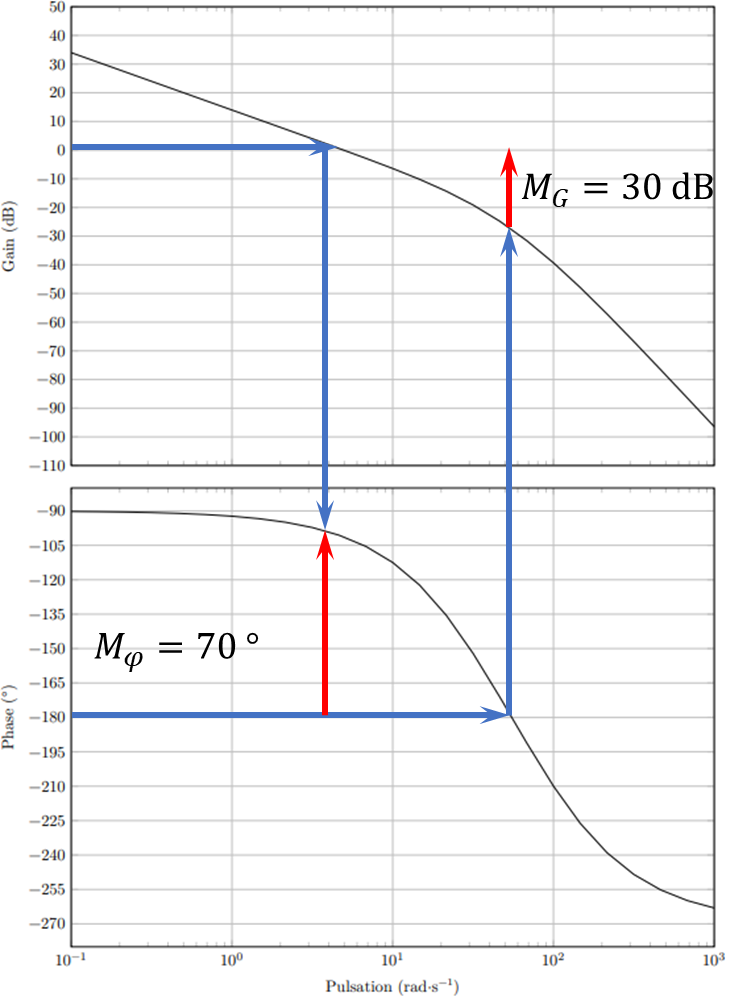
\includegraphics{Q31}
\end{center}
\end{UPSTIcorrige}

\section{Synthèse}

%Q 32. 
\UPSTIquestion Commenter les figures 14 et 15. Conclure sur le respect du cahier des charges avec les lois de commande
considérées, vis-à-vis de la stabilité du patient et du type de comportement de rééducation de l’exosquelette.

\begin{UPSTIcorrige}

\end{UPSTIcorrige}



\end{document}
